% Drawing 154/07-14 -- folder 154, batch 07, archive page 137 (PDF page 138).
% Transcription: dessins en couleur : un grand demi-disque orange rempli de pseudo-droites orange, avec, le long de sa base, un fuseau (tirets vert foncé, droite vert clair, tirets bruns) entre deux sommets marqués $1$, $2$ et des flèches de rotation ; en haut à droite, une bande étroite (vert foncé et vert clair) coupée de croisements orange, les arcs numérotés $1$ à $5$, et aux bouts « $2 : 5$ » ; une étoile au crayon avec deux sommets entourés (vert et vert foncé) et des tirets numérotés $1$, $2$ ; des croquis au crayon ; un croisement orange sur un chemin en tirets bruns ; en bas à droite, un long fuseau entre deux croisements orange, bordé de vert foncé et de vert clair, traversé de croisements orange de plus en plus serrés, un chemin en tirets bruns par les sommets, avec la légende « fuseau de croisement »
% Kind: large orange half-disk with a spindle along its base; small spindles; pencil sketches; crossing spindle. Method 2 (schematic redraw from the facsimile). Status: partial.
% Notes: Colour drawings, read from the page view: a large orange half-disk filled with orange pseudolines, along its base a spindle (dark green dashes, light green line, brown dashes) between two vertices marked 1, 2, with rotation arrows; top right a small spindle crossed by orange crossings, ends marked 2:5; a pencil star with arrows and two circled points marked by dashed numbers 1, 2; a circled point on a pencil line; bottom, a dashed line with an orange cross and a long spindle (light and dark green) crossed by orange strokes and crosses, legend « fuseau de croisement ». The strands in the half-disk are schematic; the pencilled lines at the bottom left are text of the transcription.
% Coordinates: 1 unit = 1 mm = 1/100 of the crop width (bbox in page fractions: [0.148, 0.082, 0.927, 0.489]).
% Redrawn by Claude (claude-opus-5-5), issue #73, 2026-11-07; not checked by a human; not compiled (no TeX in the session).
% Rights: reproduces part of the work -- behind RENDER_TRANSCRIPTS, never published by itself.
\documentclass[tikz,border=3pt]{standalone}
\usepackage{amsmath,amssymb}
\usetikzlibrary{patterns,arrows.meta}
\tikzset{Or/.style={orange!90!black}, Ye/.style={yellow!80!orange}, Lg/.style={green!60!black!70}, Dg/.style={green!45!black}, Br/.style={brown!80!black}, Rd/.style={red!85!black}, Bl/.style={blue!70!black}, Gy/.style={black!40}, pencil/.style={black!45}, struck/.style={black!35}, mark/.style={circle,draw,inner sep=1.3pt}, pt/.style={circle,fill,inner sep=0.9pt}, opt/.style={circle,draw,fill=white,inner sep=1.1pt}}
\begin{document}
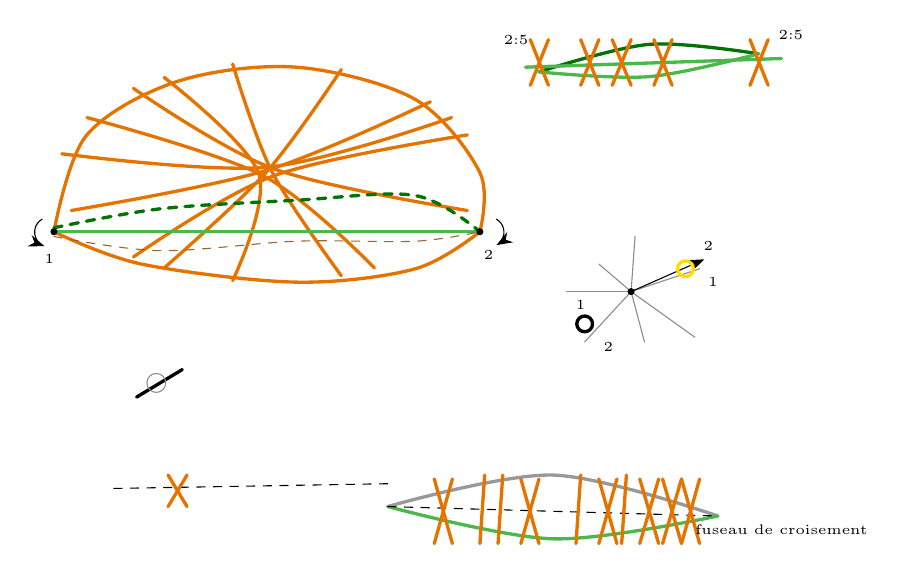
\begin{tikzpicture}[x=1mm,y=1mm,line cap=round,line join=round,font=\scriptsize]
\draw[Or,very thick] plot[smooth, tension=0.55] coordinates {(2.9,-26.7) (7,-14.5) (18.6,-7.6) (33.7,-5.8) (48.8,-9.9) (57,-19.2) (57,-26.7)};
\draw[Or,very thick] plot[smooth, tension=0.55] coordinates {(2.9,-26.7) (14,-30.8) (33.7,-33.1) (48.8,-31.4) (57,-26.7)};
\draw[Or,very thick] plot[smooth, tension=0.55] coordinates {(3.9,-16.8) (30,-18.5) (53.4,-12.2)};
\draw[Or,very thick] plot[smooth, tension=0.55] coordinates {(7.1,-12.2) (29.5,-19.6) (43.6,-31.3)};
\draw[Or,very thick] plot[smooth, tension=0.55] coordinates {(16.9,-7.1) (28.9,-19.3) (25.6,-32.9)};
\draw[Or,very thick] plot[smooth, tension=0.55] coordinates {(25.6,-5.4) (30.6,-19.1) (39.4,-32.3)};
\draw[Or,very thick] plot[smooth, tension=0.55] coordinates {(39.4,-6.1) (29.9,-19.1) (16.9,-31.3)};
\draw[Or,very thick] plot[smooth, tension=0.55] coordinates {(50.7,-10.2) (29.9,-18.9) (5.1,-24)};
\draw[Or,very thick] plot[smooth, tension=0.55] coordinates {(55.4,-14.4) (30.8,-19.6) (13,-29.9)};
\draw[Or,very thick] plot[smooth, tension=0.55] coordinates {(13,-8.5) (30.8,-18.7) (55.4,-24)};
\draw[Lg,very thick] (2.9,-26.7) -- (57,-26.7);
\draw[Dg,dashed,very thick] plot[smooth, tension=0.55] coordinates {(2.9,-26.2) (16.3,-23.8) (33.7,-22.7) (48.8,-22.1) (57,-26.7)};
\draw[Br,dashed] plot[smooth, tension=0.55] coordinates {(2.9,-27.3) (16.3,-29.1) (33.7,-27.9) (48.8,-27.9) (57,-26.7)};
\node[pt] at (2.9,-26.7) {};
\node[pt] at (57,-26.7) {};
\node[inner sep=1pt] at (2.3,-30.2) {\tiny $1$};
\node[inner sep=1pt] at (58.1,-29.7) {\tiny $2$};
\draw[-{Stealth[length=2mm]}] (1.4,-25.1) arc[start angle=120, end angle=250, x radius=1.9, y radius=1.9];
\draw[-{Stealth[length=2mm]}] (59.1,-25.1) arc[start angle=60, end angle=-60, x radius=1.9, y radius=1.9];
\draw[Dg,very thick] plot[smooth, tension=0.55] coordinates {(64.5,-6.4) (78.5,-2.9) (92.4,-4.1)};
\draw[Lg,very thick] plot[smooth, tension=0.55] coordinates {(64.5,-6.4) (78.5,-7) (92.4,-4.1)};
\draw[Lg,very thick] (62.8,-5.8) -- (95.3,-4.7);
\draw[Or,very thick] (63.4,-2.3) -- (65.7,-8.1);
\draw[Or,very thick] (65.7,-2.3) -- (63.4,-8.1);
\draw[Or,very thick] (69.8,-2.3) -- (72.1,-8.1);
\draw[Or,very thick] (72.1,-2.3) -- (69.8,-8.1);
\draw[Or,very thick] (73.8,-2.3) -- (76.2,-8.1);
\draw[Or,very thick] (76.2,-2.3) -- (73.8,-8.1);
\draw[Or,very thick] (79.1,-2.3) -- (81.4,-8.1);
\draw[Or,very thick] (81.4,-2.3) -- (79.1,-8.1);
\draw[Or,very thick] (91.3,-2.3) -- (93.6,-8.1);
\draw[Or,very thick] (93.6,-2.3) -- (91.3,-8.1);
\node[inner sep=1pt] at (61.6,-2.3) {\tiny $2{:}5$};
\node[inner sep=1pt] at (96.5,-1.7) {\tiny $2{:}5$};
\draw[pencil] (76.2,-34.3) -- (72.1,-30.8);
\draw[pencil] (76.2,-34.3) -- (76.7,-27.3);
\draw[pencil] (76.2,-34.3) -- (84.9,-31.4);
\draw[pencil] (76.2,-34.3) -- (84.3,-40.1);
\draw[pencil] (76.2,-34.3) -- (70.3,-40.7);
\draw[pencil] (76.2,-34.3) -- (68,-34.3);
\draw[pencil] (76.2,-34.3) -- (77.9,-40.7);
\node[pt] at (76.2,-34.3) {};
\draw[-{Stealth[length=2mm]}] (76.2,-34.3) -- (85.5,-30.2);
\draw[Ye,very thick] (83.1,-31.4) circle[radius=1];
\draw[very thick] (70.3,-38.4) circle[radius=1];
\node[inner sep=1pt] at (86,-28.5) {\tiny $2$};
\node[inner sep=1pt] at (86.6,-33.1) {\tiny $1$};
\node[inner sep=1pt] at (69.8,-36) {\tiny $1$};
\node[inner sep=1pt] at (73.3,-41.3) {\tiny $2$};
\draw[very thick] (13.4,-47.7) -- (19.2,-44.2);
\draw[pencil] (15.9,-45.9) circle[radius=1.2];
\draw[dashed] (10.5,-59.3) -- (45.3,-58.7);
\draw[Or,very thick] (17.4,-57.6) -- (19.8,-61.6);
\draw[Or,very thick] (19.8,-57.6) -- (17.4,-61.6);
\draw[Gy,very thick] plot[smooth, tension=0.55] coordinates {(45.3,-61.6) (66.3,-57.6) (87.2,-62.8)};
\draw[Lg,very thick] plot[smooth, tension=0.55] coordinates {(45.3,-61.6) (66.3,-65.7) (87.2,-62.8)};
\draw[dashed] (45.3,-61.6) -- (87.2,-62.8);
\draw[Or,very thick] (57.6,-57.6) -- (57,-66.3);
\draw[Or,very thick] (59.9,-57.6) -- (59.3,-66.3);
\draw[Or,very thick] (69.8,-57.6) -- (69.2,-66.3);
\draw[Or,very thick] (75.6,-57.6) -- (75,-66.3);
\draw[Or,very thick] (51.2,-58.1) -- (53.5,-66.3);
\draw[Or,very thick] (53.5,-58.1) -- (51.2,-66.3);
\draw[Or,very thick] (62.2,-58.1) -- (64.5,-66.3);
\draw[Or,very thick] (64.5,-58.1) -- (62.2,-66.3);
\draw[Or,very thick] (72.1,-58.1) -- (74.4,-66.3);
\draw[Or,very thick] (74.4,-58.1) -- (72.1,-66.3);
\draw[Or,very thick] (77.3,-58.1) -- (79.7,-66.3);
\draw[Or,very thick] (79.7,-58.1) -- (77.3,-66.3);
\draw[Or,very thick] (80.2,-58.1) -- (82.6,-66.3);
\draw[Or,very thick] (82.6,-58.1) -- (80.2,-66.3);
\draw[Or,very thick] (82.6,-58.1) -- (84.9,-66.3);
\draw[Or,very thick] (84.9,-58.1) -- (82.6,-66.3);
\node[inner sep=1pt] at (95.3,-64.5) {\tiny fuseau de croisement};
\end{tikzpicture}
\end{document}
